\begin{landscape}
\section{Data Class Diagram}
Di seguito viene riportato il diagramma delle classi che rappresenta la struttura del database e delle entità presenti nell'applicazione.

\begin{figure}[h!]
	\centering
	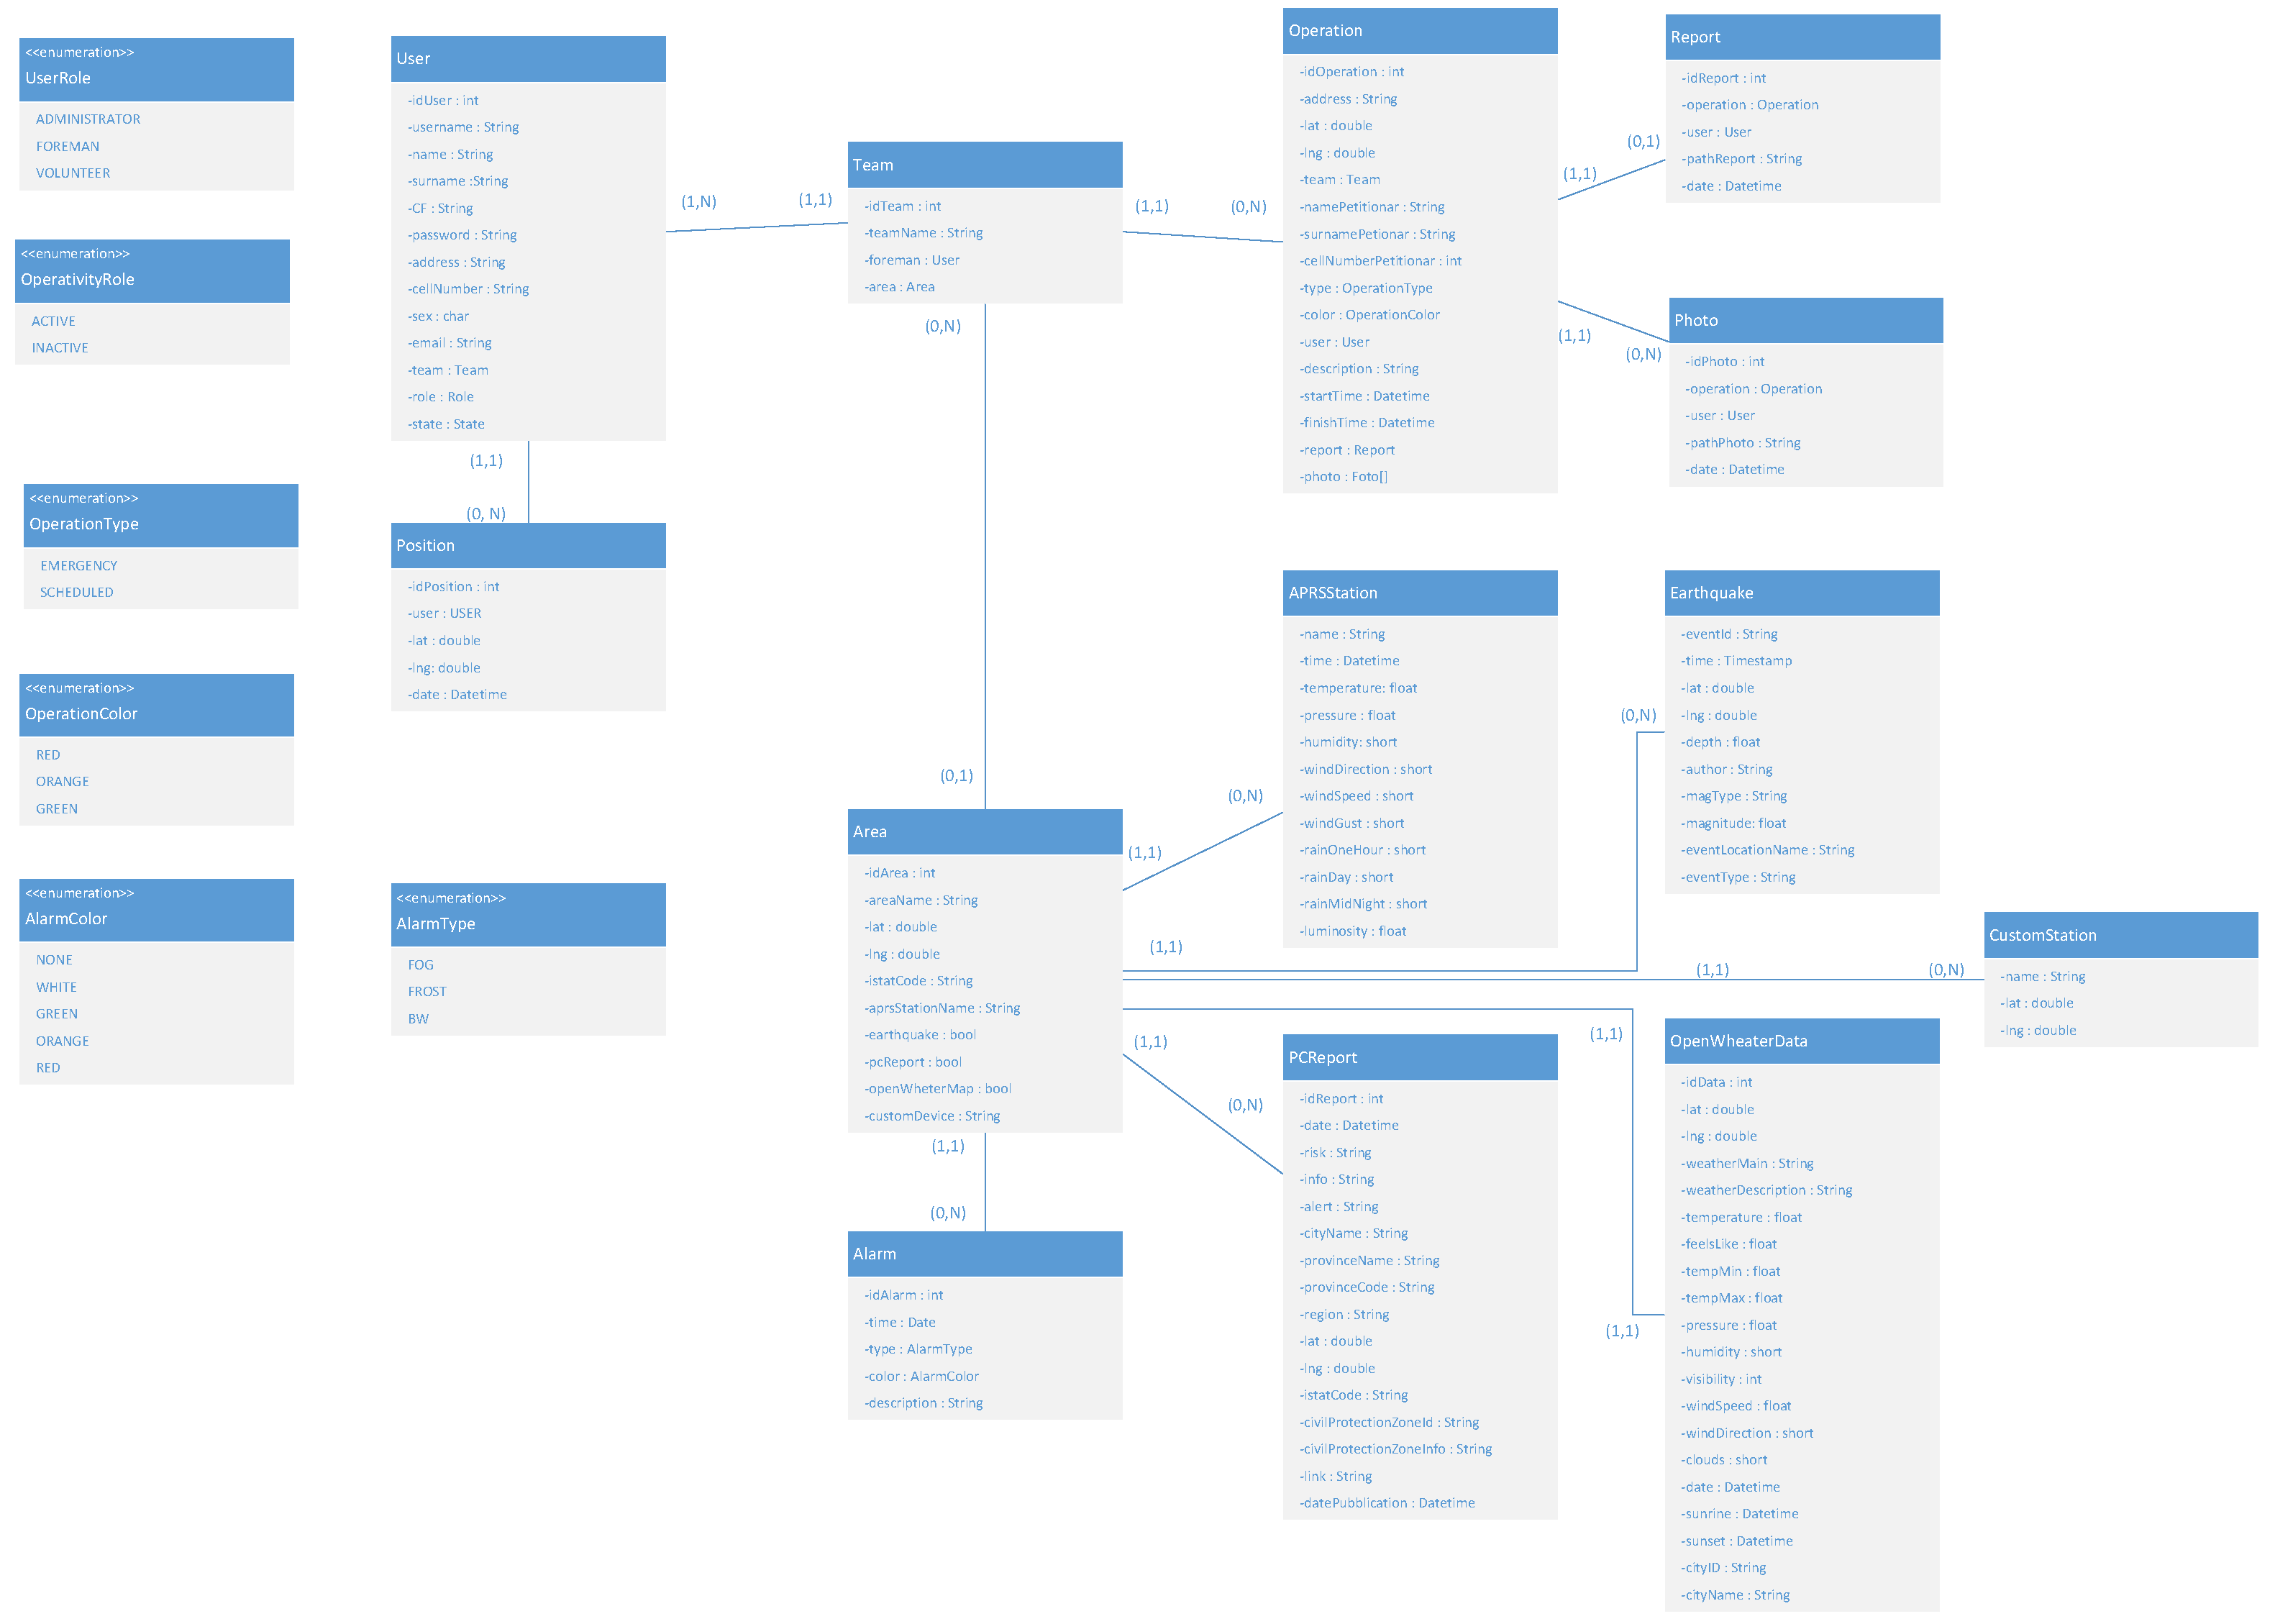
\includegraphics[width=0.8\linewidth]{./Iterazione 1/OtherFiles/UML - Data Class View}
	\caption{Data Class Diagram.}
	\label{fig:DataClassDiagram}
\end{figure}
\end{landscape}